\begin{figure}
	\centering
	\pgfplotsset{every axis legend/.append style={
		at={(1.05,0.5)},
		anchor=west}}
	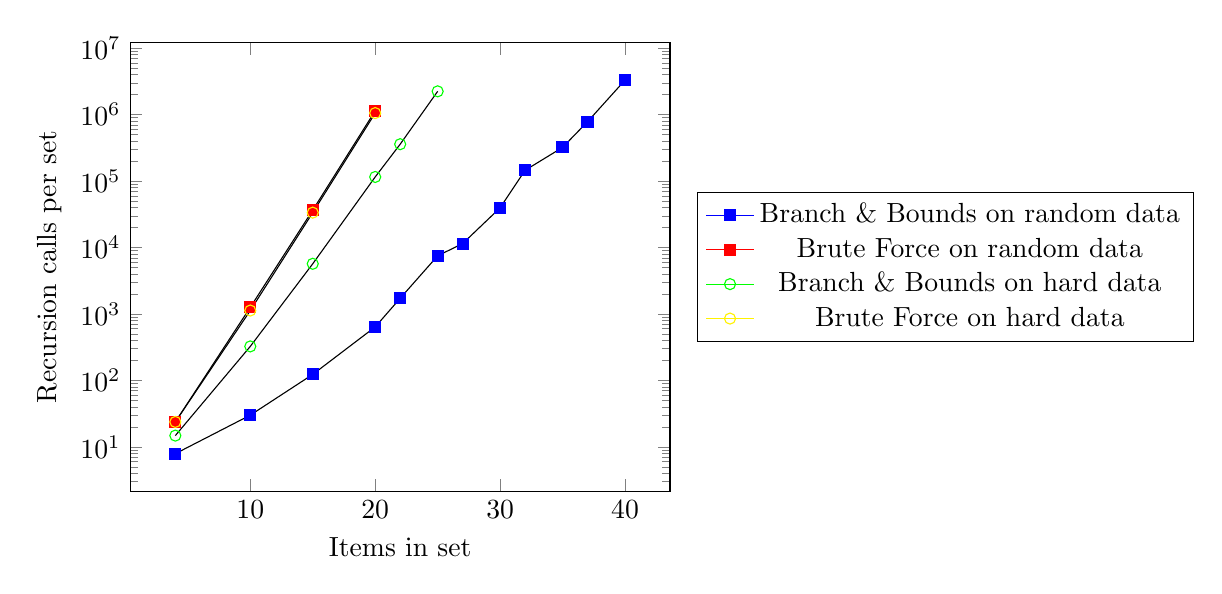
\begin{tikzpicture}
		\begin{semilogyaxis}[
			xlabel=Items in set,
			ylabel=Recursion calls per set,
			scatter/classes={
				NSm={mark=square*,blue},
				NSt={mark=square*,red},
				ZSm={mark=o,draw=green},
				ZSt={mark=o,draw=yellow}
				}
			]
			\addplot[scatter,%
				scatter src=explicit symbolic]%
			table[meta=label] {
				x y label
				4 23.71 NSt
				10 1258.43 NSt
				15 36477.82 NSt
				20 1139944.81 NSt
			};
			\addplot[scatter,%
				scatter src=explicit symbolic]%
			table[meta=label] {
				x y label
				4 7.88 NSm
				10 29.96 NSm
				15 122.98 NSm
				20 637.70 NSm
				22 1718.99 NSm
				25 7495.38 NSm
				27 11446.80 NSm
				30 39577.47 NSm
				32 145111.69 NSm
				35 320850.22 NSm
				37 782664.08 NSm
				40 3304721.06 NSm
			};
			\addplot[scatter,%
				scatter src=explicit symbolic]%
			table[meta=label] {
				x y label
				4 23.70 ZSt
				10 1125.09 ZSt
				15 33469.84 ZSt
				20 1054059.56 ZSt
			};
			\addplot[scatter,%
				scatter src=explicit symbolic]%
			table[meta=label] {
				x y label
				4 14.75 ZSm
				10 324.50 ZSm
				15 5685.97 ZSm
				20 115219.09 ZSm
				22 358548.04 ZSm
				25 2238413.90 ZSm
			};
			\addlegendentry{Branch \& Bounds on random data}
			\addlegendentry{Brute Force on random data}
			\addlegendentry{Branch \& Bounds on hard data}
			\addlegendentry{Brute Force on hard data}
		\end{semilogyaxis}
	\end{tikzpicture}
\caption{Number of recursion calls depending on number of items in set}
\label{plot:fullCalls}
\end{figure}